\chapter{Diagrammes internes de blocs (ibd)}
Le \textbf{Système élévateur} associé aux meubles permettant d'adapter la hauteurs de ces derniers à celle de l'habitant fonctionne de la façon présentée ci-dessous.

Le système reçoit deux paramètres: la hauteur de l'habitant \textbf{\textit{hauteurHabitant}} (nulle si personne est dans la douche) et une valeur booléenne \textbf{\textit{estDansLaDouche}}indiquant si l'utilisateur se trouve dans la douche. 
La hauteur de l'habitant est transmise au \textbf{Contrôleur} qui va à son tour récupérer la position du mobilier, c'est-à-dire sa hauteur \textbf{\textit{hauteurMobilier}} par rapport au sol. Il va comparer cette valeur obtenue à la hauteur de l'habitant récupérée en entrée afin de déterminer la position de la dalle élévatrice \textbf{\textit{positionDalle}}. 
\begin{figure}[H]
	\centering
	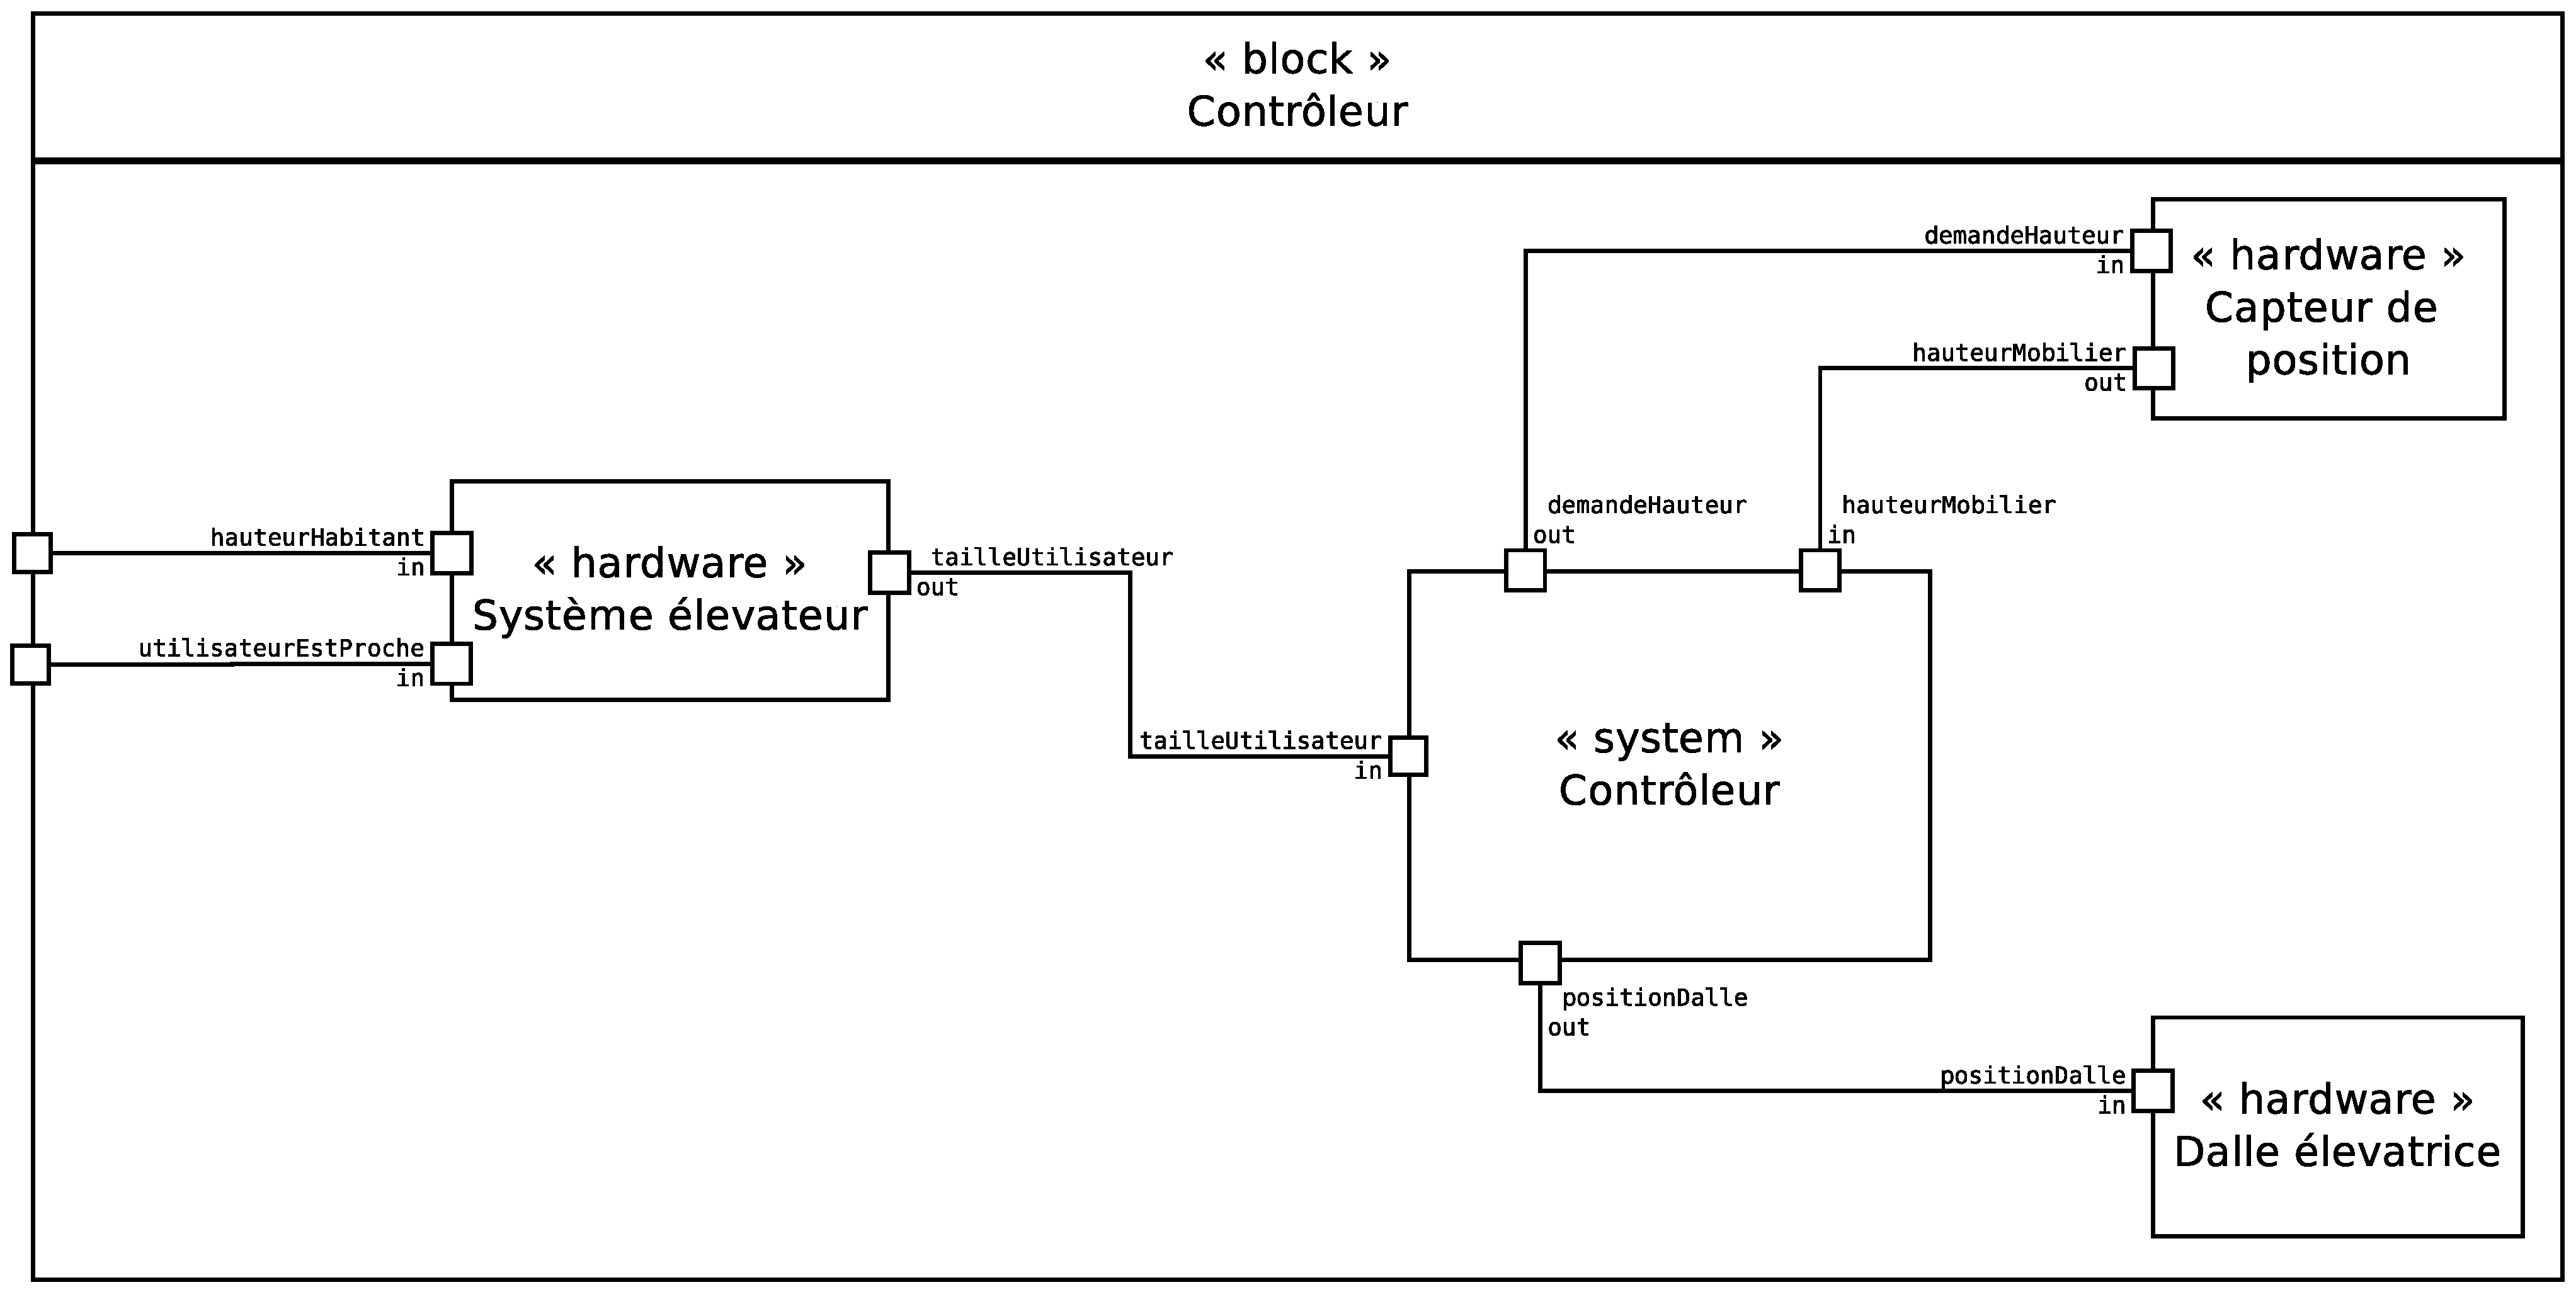
\includegraphics[width=1\linewidth]{diagrams/bathroom/diagramme_blocks_ibd.eps}
	\caption{Diagramme interne de blocs pour actionner la montée-descente d'un mobilier}
	\label{fig:diagramme_ibd}
\end{figure}
